\section{Wasserstein重心}
\label{sec:ot-barycenter}

上一节在两个分布之间取中途状态。有多个分布时，能否找一个分布共同代表它们？对点$x_1,\dots,x_K\in\mathbb{R}^{d}$与权重$\lambda_k$，加权平均$\bar{x}=\sum_k\lambda_kx_k$是使$\sum_k\lambda_k\lVert y-x_k\rVert_2^{2}$最小的点。把点换成分布、把平方距离换成$W_2^{2}$，就得到分布的“平均”。

\begin{definition}[Wasserstein重心]
\label{def:ot-barycenter}
设$\mu_1,\dots,\mu_K$是$\mathbb{R}^{d}$上具有有限二阶矩的分布，权重$\lambda_k\geq0$，$\sum_k\lambda_k=1$。在有限二阶矩的分布$\nu$中最小化
\begin{equation}
 \Psi(\nu)=\sum_{k=1}^{K}\lambda_kW_2^{2}(\nu,\mu_k),
 \label{eq:ot-barycenter}
\end{equation}
最小点称为$\mu_1,\dots,\mu_K$关于这组权重的\term{Wasserstein重心}（Wasserstein barycenter）。
\end{definition}

它与混合分布$\sum_k\lambda_k\mu_k$是两回事。混合把各分布的质量按权重叠在一起，质量都留在原处；重心则把质量搬到“平均位置”上。

\paragraph{点质量的重心}
取$\mu_k=\delta_{x_k}$。任何$\nu$与点质量只有一个耦合，即$\nu\otimes\delta_{x_k}$，所以
\[
 W_2^{2}(\nu,\delta_{x_k})=\int\lVert y-x_k\rVert_2^{2}\,\nu(\mathrm{d}y).
\]对每个$y$有恒等式
\[
 \sum_k\lambda_k\lVert y-x_k\rVert_2^{2}=\lVert y-\bar{x}\rVert_2^{2}+\sum_k\lambda_k\lVert x_k-\bar{x}\rVert_2^{2},
\]
因为交叉项$2\sum_k\lambda_k\langle y-\bar{x},\bar{x}-x_k\rangle$中$\sum_k\lambda_k(\bar{x}-x_k)=0$。对$\nu$积分，
\[
 \Psi(\nu)=\int\lVert y-\bar{x}\rVert_2^{2}\,\nu(\mathrm{d}y)+\sum_k\lambda_k\lVert x_k-\bar{x}\rVert_2^{2},
\]
第一项在且仅在$\nu=\delta_{\bar{x}}$时为零。所以点质量的重心唯一，是$\delta_{\bar{x}}$，正是点的加权平均；混合分布$\sum_k\lambda_k\delta_{x_k}$则在每个$x_k$上各放一份质量。

\paragraph{两个分布的重心}
$K=2$、权重$(1-t,t)$时，位移插值$\mu_t$是重心。记$W=W_2(\mu_0,\mu_1)$，任取$\nu$，令$\alpha=W_2(\nu,\mu_0)$，$\beta=W_2(\nu,\mu_1)$，由三角不等式$\alpha+\beta\geq W$。直接展开可以验证
\[
 (1-t)\alpha^{2}+t\beta^{2}-t(1-t)(\alpha+\beta)^{2}=\bigl((1-t)\alpha-t\beta\bigr)^{2}\geq0 ,
\]
所以$\Psi(\nu)\geq t(1-t)W^{2}$。由定理~\ref{thm:ot-geodesic}，$\mu_t$满足$\alpha=tW$，$\beta=(1-t)W$，代入得
\[
 \Psi(\mu_t)=(1-t)t^{2}W^{2}+t(1-t)^{2}W^{2}=t(1-t)W^{2},
\]
达到下界。

\paragraph{实数轴上的重心}
一维时，由定理~\ref{thm:ot-one-dimensional}，$W_2^{2}$是分位数函数之差的平方积分，重心问题化为分位数函数的最小二乘。

\begin{theorem}[一维重心]
\label{thm:ot-barycenter-1d}
设$\mu_1,\dots,\mu_K$是实数轴上具有有限二阶矩的分布，分位数函数为$F_k^{-1}$。则重心唯一，它的分位数函数是
\begin{equation}
 \bar{q}(u)=\sum_{k=1}^{K}\lambda_kF_k^{-1}(u),\qquad0<u<1 .
 \label{eq:ot-barycenter-1d}
\end{equation}
\end{theorem}

\begin{proof}
任取有限二阶矩的分布$\nu$，分位数函数为$G^{-1}$。由式~\eqref{eq:ot-quantile-formula}与点质量情形中的同一恒等式（逐个$u$使用），
\[
 \Psi(\nu)=\int_0^{1}\bigl(G^{-1}(u)-\bar{q}(u)\bigr)^{2}\,\mathrm{d}u+\sum_k\lambda_k\int_0^{1}\bigl(F_k^{-1}(u)-\bar{q}(u)\bigr)^{2}\,\mathrm{d}u .
\]
第二项与$\nu$无关。$\bar{q}$是单调不减、左连续函数的非负组合，仍单调不减且左连续；由各$F_k^{-1}$平方可积，它也平方可积。令$\bar{\nu}$为$\bar{q}(U)$的分布，$U\sim\operatorname{Unif}(0,1)$，由单调性与左连续性可以验证$\bar{\nu}$的分位数函数就是$\bar{q}$，并且$\bar{\nu}$有有限二阶矩。于是$\bar{\nu}$使第一项为零，是重心。反过来，任何重心都使第一项为零，$G^{-1}=\bar{q}$几乎处处成立；两个左连续单调函数几乎处处相等就处处相等，所以重心就是$\bar{\nu}$。
\end{proof}

对一维高斯分布$\mu_k=\mathcal{N}(m_k,\sigma_k^{2})$，$F_k^{-1}(u)=m_k+\sigma_k\Phi^{-1}(u)$，其中$\Phi$是标准高斯分布函数，于是重心是
\[
 \mathcal{N}\Bigl(\sum_k\lambda_km_k,\ \bigl(\textstyle\sum_k\lambda_k\sigma_k\bigr)^{2}\Bigr):
\]
均值平均，标准差也平均。图~\ref{fig:ot-barycenter}取三个形状不同的分布，$\mathcal{N}(-3,0.5^{2})$、$\operatorname{Unif}(-1,1)$与$\mathcal{N}(3.5,0.8^{2})$，权重各$\tfrac13$。重心的分位数函数是
\[
 \bar{q}(u)=\tfrac13\bigl(-0.5+1.3\,\Phi^{-1}(u)+2u\bigr),
\]
均值为$\tfrac16$，形状介于高斯与均匀之间，是一个单峰分布；混合分布则保留三个分开的峰。

\begin{BookInlineFigure}
 \centering
 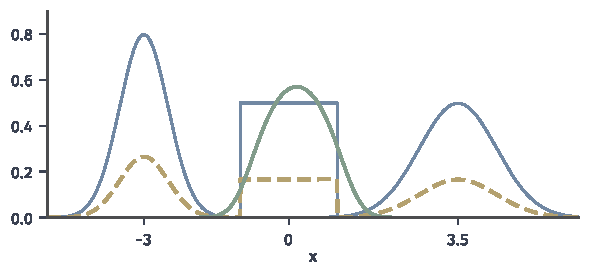
\includegraphics[width=100mm]{figures/07-probability/07-distribution-optimization/matplotlib/ot-barycenter/figure.pdf}
 \caption{三个分布（蓝）：$\mathcal{N}(-3,0.5^{2})$、$\operatorname{Unif}(-1,1)$、$\mathcal{N}(3.5,0.8^{2})$，权重各$\tfrac13$。绿线是Wasserstein重心的密度，由平均分位数函数式~\eqref{eq:ot-barycenter-1d}数值求得；黄色虚线是混合分布的密度。}
 \label{fig:ot-barycenter}
\end{BookInlineFigure}

\paragraph{存在与唯一}
一般维数中没有分位数可用，但存在性可以沿用第~\ref{sec:ot-existence}节的紧性论证。

\begin{theorem}[重心的存在]
\label{thm:ot-barycenter-existence}
在定义~\ref{def:ot-barycenter}的条件下，重心存在。
\end{theorem}

\begin{proof}
记$V=\inf_\nu\Psi(\nu)$，取$\nu=\mu_1$知$V<\infty$。取有限二阶矩的分布列$\nu_l$，使$\Psi(\nu_l)\to V$。

\emph{二阶矩一致有界。}取$\lambda_{k_0}>0$。$\lVert y\rVert_2^{2}$不超过$2\lVert y-x\rVert_2^{2}+2\lVert x\rVert_2^{2}$，在$\nu_l$与$\mu_{k_0}$的最优耦合下取期望，
\[
 \int\lVert y\rVert_2^{2}\,\nu_l(\mathrm{d}y)\leq\frac{2\Psi(\nu_l)}{\lambda_{k_0}}+2\int\lVert x\rVert_2^{2}\,\mu_{k_0}(\mathrm{d}x),
\]
右边对$l$有界，记为$M$。由第~\ref{chap:weak-convergence-of-distributions}章的矩条件，$\{\nu_l\}$胎紧，有子列（仍记为$\nu_l$）弱收敛到某个$\nu$。对每个$R>0$，$\min(\lVert y\rVert_2^{2},R)$有界连续，其积分在极限中不超过$M$；令$R\to\infty$，$\nu$的二阶矩不超过$M$。

\emph{距离下半连续。}固定$k$，取子列使$W_2^{2}(\nu_l,\mu_k)$趋于它的下极限，取最优耦合$\pi_l\in\Pi(\nu_l,\mu_k)$。$\{\nu_l\}$与$\mu_k$都胎紧，按引理~\ref{lem:ot-coupling-compact}的证明，$\{\pi_l\}$胎紧，再取子列使$\pi_l\xrightarrow{\mathrm{w}}\pi$。对有界连续的$h$，
\[
 \int h(x)\,\pi(\mathrm{d}x,\mathrm{d}y)=\lim_{l\to\infty}\int h\,\mathrm{d}\nu_l=\int h\,\mathrm{d}\nu ,
\]
所以$\pi$的第一边缘是$\nu$；每个$\pi_l$的第二边缘都是$\mu_k$，同样的论证说明$\pi$的第二边缘也是$\mu_k$。由引理~\ref{lem:ot-cost-lsc}，
\[
 W_2^{2}(\nu,\mu_k)\leq\int\lVert x-y\rVert_2^{2}\,\mathrm{d}\pi\leq\liminf_{l\to\infty}W_2^{2}(\nu_l,\mu_k).
\]
对$k$加权求和，下极限之和不超过和的下极限，于是$\Psi(\nu)\leq\liminf_l\Psi(\nu_l)=V$。
\end{proof}

唯一性需要额外条件。若某个权重为正的$\mu_k$关于Lebesgue测度绝对连续，重心唯一。机制是：这时$\nu\mapsto W_2^{2}(\nu,\mu_k)$在分布的混合下严格凸，而$\Psi$的其余各项是凸的；严格凸性来自第~\ref{sec:ot-interpolation}节提到的最优耦合由凸函数梯度唯一给出，证明可查阅前面提到的Villani的专著。条件不能随意去掉。在第~\ref{sec:ot-interpolation}节的正方形例子中取权重$(\tfrac12,\tfrac12)$，两个分布都是点质量组成的，不绝对连续；三种不同的中途状态都满足$\alpha=\beta=\tfrac12W$，都使$\Psi$达到下界$\tfrac14W^{2}$，所以重心不唯一。一维情形是例外，定理~\ref{thm:ot-barycenter-1d}对任何有限二阶矩的分布都给出唯一性。
